\documentclass[1p]{elsarticle_modified}
%\bibliographystyle{elsarticle-num}

%\usepackage[colorlinks]{hyperref}
%\usepackage{abbrmath_seonhwa} %\Abb, \Ascr, \Acal ,\Abf, \Afrak
\usepackage{amsfonts}
\usepackage{amssymb}
\usepackage{amsmath}
\usepackage{amsthm}
\usepackage{scalefnt}
\usepackage{amsbsy}
\usepackage{kotex}
\usepackage{caption}
\usepackage{subfig}
\usepackage{color}
\usepackage{graphicx}
\usepackage{xcolor} %% white, black, red, green, blue, cyan, magenta, yellow
\usepackage{float}
\usepackage{setspace}
\usepackage{hyperref}

\usepackage{tikz}
\usetikzlibrary{arrows}

\usepackage{multirow}
\usepackage{array} % fixed length table
\usepackage{hhline}

%%%%%%%%%%%%%%%%%%%%%
\makeatletter
\renewcommand*\env@matrix[1][\arraystretch]{%
	\edef\arraystretch{#1}%
	\hskip -\arraycolsep
	\let\@ifnextchar\new@ifnextchar
	\array{*\c@MaxMatrixCols c}}
\makeatother %https://tex.stackexchange.com/questions/14071/how-can-i-increase-the-line-spacing-in-a-matrix
%%%%%%%%%%%%%%%

\usepackage[normalem]{ulem}

\newcommand{\msout}[1]{\ifmmode\text{\sout{\ensuremath{#1}}}\else\sout{#1}\fi}
%SOURCE: \msout is \stkout macro in https://tex.stackexchange.com/questions/20609/strikeout-in-math-mode

\newcommand{\cancel}[1]{
	\ifmmode
	{\color{red}\msout{#1}}
	\else
	{\color{red}\sout{#1}}
	\fi
}

\newcommand{\add}[1]{
	{\color{blue}\uwave{#1}}
}

\newcommand{\replace}[2]{
	\ifmmode
	{\color{red}\msout{#1}}{\color{blue}\uwave{#2}}
	\else
	{\color{red}\sout{#1}}{\color{blue}\uwave{#2}}
	\fi
}

\newcommand{\Sol}{\mathcal{S}} %segment
\newcommand{\D}{D} %diagram
\newcommand{\A}{\mathcal{A}} %arc


%%%%%%%%%%%%%%%%%%%%%%%%%%%%%5 test

\def\sl{\operatorname{\textup{SL}}(2,\Cbb)}
\def\psl{\operatorname{\textup{PSL}}(2,\Cbb)}
\def\quan{\mkern 1mu \triangleright \mkern 1mu}

\theoremstyle{definition}
\newtheorem{thm}{Theorem}[section]
\newtheorem{prop}[thm]{Proposition}
\newtheorem{lem}[thm]{Lemma}
\newtheorem{ques}[thm]{Question}
\newtheorem{cor}[thm]{Corollary}
\newtheorem{defn}[thm]{Definition}
\newtheorem{exam}[thm]{Example}
\newtheorem{rmk}[thm]{Remark}
\newtheorem{alg}[thm]{Algorithm}

\newcommand{\I}{\sqrt{-1}}
\begin{document}

%\begin{frontmatter}
%
%\title{Boundary parabolic representations of knots up to 8 crossings}
%
%%% Group authors per affiliation:
%\author{Yunhi Cho} 
%\address{Department of Mathematics, University of Seoul, Seoul, Korea}
%\ead{yhcho@uos.ac.kr}
%
%
%\author{Seonhwa Kim} %\fnref{s_kim}}
%\address{Center for Geometry and Physics, Institute for Basic Science, Pohang, 37673, Korea}
%\ead{ryeona17@ibs.re.kr}
%
%\author{Hyuk Kim}
%\address{Department of Mathematical Sciences, Seoul National University, Seoul 08826, Korea}
%\ead{hyukkim@snu.ac.kr}
%
%\author{Seokbeom Yoon}
%\address{Department of Mathematical Sciences, Seoul National University, Seoul, 08826,  Korea}
%\ead{sbyoon15@snu.ac.kr}
%
%\begin{abstract}
%We find all boundary parabolic representation of knots up to 8 crossings.
%
%\end{abstract}
%\begin{keyword}
%    \MSC[2010] 57M25 
%\end{keyword}
%
%\end{frontmatter}

%\linenumbers
%\tableofcontents
%
\newcommand\colored[1]{\textcolor{white}{\rule[-0.35ex]{0.8em}{1.4ex}}\kern-0.8em\color{red} #1}%
%\newcommand\colored[1]{\textcolor{white}{ #1}\kern-2.17ex	\textcolor{white}{ #1}\kern-1.81ex	\textcolor{white}{ #1}\kern-2.15ex\color{red}#1	}

{\Large $\underline{12n_{0464}~(K12n_{0464})}$}

\setlength{\tabcolsep}{10pt}
\renewcommand{\arraystretch}{1.6}
\vspace{1cm}\begin{tabular}{m{100pt}>{\centering\arraybackslash}m{274pt}}
\multirow{5}{120pt}{
	\centering
	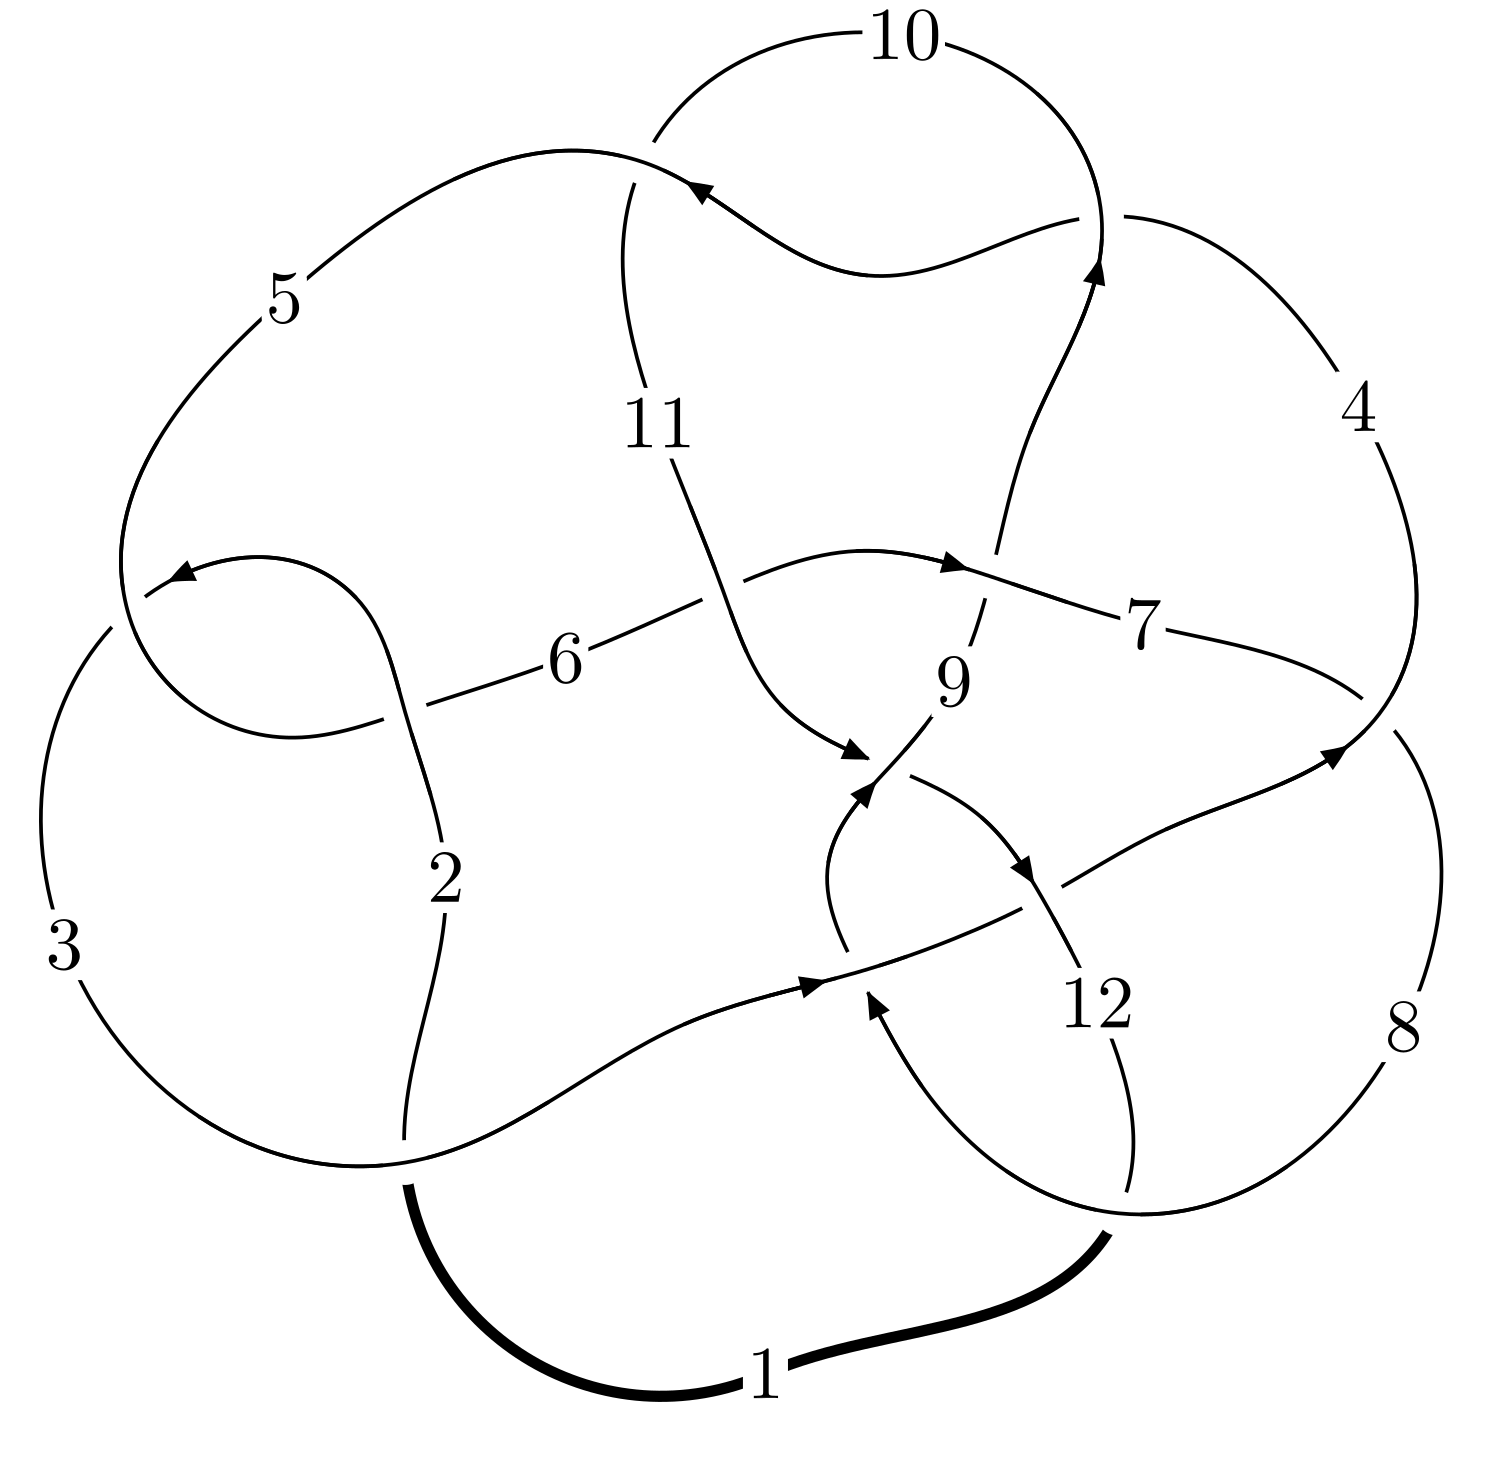
\includegraphics[width=112pt]{../../../GIT/diagram.site/Diagrams/png/2553_12n_0464.png}\\
\ \ \ A knot diagram\footnotemark}&
\allowdisplaybreaks
\textbf{Linearized knot diagam} \\
\cline{2-2}
 &
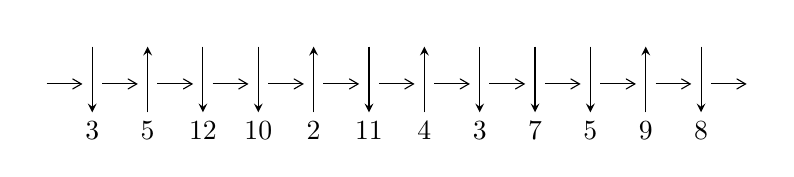
\begin{tikzpicture}[x=20pt, y=17pt]
	% nodes
	\node (C0) at (0, 0) {};
	\node (C1) at (1, 0) {};
	\node (C1U) at (1, +1) {};
	\node (C1D) at (1, -1) {3};

	\node (C2) at (2, 0) {};
	\node (C2U) at (2, +1) {};
	\node (C2D) at (2, -1) {5};

	\node (C3) at (3, 0) {};
	\node (C3U) at (3, +1) {};
	\node (C3D) at (3, -1) {12};

	\node (C4) at (4, 0) {};
	\node (C4U) at (4, +1) {};
	\node (C4D) at (4, -1) {10};

	\node (C5) at (5, 0) {};
	\node (C5U) at (5, +1) {};
	\node (C5D) at (5, -1) {2};

	\node (C6) at (6, 0) {};
	\node (C6U) at (6, +1) {};
	\node (C6D) at (6, -1) {11};

	\node (C7) at (7, 0) {};
	\node (C7U) at (7, +1) {};
	\node (C7D) at (7, -1) {4};

	\node (C8) at (8, 0) {};
	\node (C8U) at (8, +1) {};
	\node (C8D) at (8, -1) {3};

	\node (C9) at (9, 0) {};
	\node (C9U) at (9, +1) {};
	\node (C9D) at (9, -1) {7};

	\node (C10) at (10, 0) {};
	\node (C10U) at (10, +1) {};
	\node (C10D) at (10, -1) {5};

	\node (C11) at (11, 0) {};
	\node (C11U) at (11, +1) {};
	\node (C11D) at (11, -1) {9};

	\node (C12) at (12, 0) {};
	\node (C12U) at (12, +1) {};
	\node (C12D) at (12, -1) {8};
	\node (C13) at (13, 0) {};

	% arrows
	\draw[->,>={angle 60}]
	(C0) edge (C1) (C1) edge (C2) (C2) edge (C3) (C3) edge (C4) (C4) edge (C5) (C5) edge (C6) (C6) edge (C7) (C7) edge (C8) (C8) edge (C9) (C9) edge (C10) (C10) edge (C11) (C11) edge (C12) (C12) edge (C13) ;	\draw[->,>=stealth]
	(C1U) edge (C1D) (C2D) edge (C2U) (C3U) edge (C3D) (C4U) edge (C4D) (C5D) edge (C5U) (C6U) edge (C6D) (C7D) edge (C7U) (C8U) edge (C8D) (C9U) edge (C9D) (C10U) edge (C10D) (C11D) edge (C11U) (C12U) edge (C12D) ;
	\end{tikzpicture} \\
\hhline{~~} \\& 
\textbf{Solving Sequence} \\ \cline{2-2} 
 &
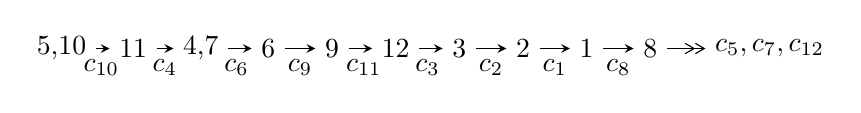
\begin{tikzpicture}[x=23pt, y=7pt]
	% node
	\node (A0) at (-1/8, 0) {5,10};
	\node (A1) at (1, 0) {11};
	\node (A2) at (33/16, 0) {4,7};
	\node (A3) at (25/8, 0) {6};
	\node (A4) at (33/8, 0) {9};
	\node (A5) at (41/8, 0) {12};
	\node (A6) at (49/8, 0) {3};
	\node (A7) at (57/8, 0) {2};
	\node (A8) at (65/8, 0) {1};
	\node (A9) at (73/8, 0) {8};
	\node (C1) at (1/2, -1) {$c_{10}$};
	\node (C2) at (3/2, -1) {$c_{4}$};
	\node (C3) at (21/8, -1) {$c_{6}$};
	\node (C4) at (29/8, -1) {$c_{9}$};
	\node (C5) at (37/8, -1) {$c_{11}$};
	\node (C6) at (45/8, -1) {$c_{3}$};
	\node (C7) at (53/8, -1) {$c_{2}$};
	\node (C8) at (61/8, -1) {$c_{1}$};
	\node (C9) at (69/8, -1) {$c_{8}$};
	\node (A10) at (11, 0) {$c_{5},c_{7},c_{12}$};

	% edge
	\draw[->,>=stealth]	
	(A0) edge (A1) (A1) edge (A2) (A2) edge (A3) (A3) edge (A4) (A4) edge (A5) (A5) edge (A6) (A6) edge (A7) (A7) edge (A8) (A8) edge (A9) ;
	\draw[->>,>={angle 60}]	
	(A9) edge (A10);
\end{tikzpicture} \\ 

\end{tabular} \\

\footnotetext{
The image of knot diagram is generated by the software ``\textbf{Draw programme}" developed by Andrew Bartholomew(\url{http://www.layer8.co.uk/maths/draw/index.htm\#Running-draw}), where we modified some parts for our purpose(\url{https://github.com/CATsTAILs/LinksPainter}).
}\phantom \\ \newline 
\centering \textbf{Ideals for irreducible components\footnotemark of $X_{\text{par}}$} 
 
\begin{align*}
I^u_{1}&=\langle 
-9 u^{10}+50 u^9-110 u^8+84 u^7+135 u^6-318 u^5+249 u^4+140 u^3+64 u^2+356 b-268 u+100,\\
\phantom{I^u_{1}}&\phantom{= \langle  }209 u^{10}-1438 u^9+\cdots+712 a+1396,\\
\phantom{I^u_{1}}&\phantom{= \langle  }u^{11}-8 u^{10}+28 u^9-48 u^8+21 u^7+72 u^6-147 u^5+118 u^4-46 u^3+12 u^2+4 u-8\rangle \\
I^u_{2}&=\langle 
- u^{13}-2 u^{12}+7 u^{11}+14 u^{10}-18 u^9-37 u^8+18 u^7+40 u^6-3 u^4-11 u^3-27 u^2+2 b+6 u+16,\\
\phantom{I^u_{2}}&\phantom{= \langle  }-16 u^{13}+125 u^{11}+\cdots+38 a-152,\;u^{14}-9 u^{12}+33 u^{10}-60 u^8+48 u^6+6 u^4-37 u^2+19\rangle \\
I^u_{3}&=\langle 
- u^2 a+a u+u^2+b- u,\;u^5 a-3 u^4 a+2 u^5+4 u^3 a-9 u^4+13 u^3+4 a^2+a u-4 u^2-8 a-6 u-7,\\
\phantom{I^u_{3}}&\phantom{= \langle  }u^6-5 u^5+10 u^4-8 u^3+u^2-2 u+4\rangle \\
\\
I^v_{1}&=\langle 
a,\;b^2+b+1,\;v+1\rangle \\
\end{align*}
\raggedright * 4 irreducible components of $\dim_{\mathbb{C}}=0$, with total 39 representations.\\
\footnotetext{All coefficients of polynomials are rational numbers. But the coefficients are sometimes approximated in decimal forms when there is not enough margin.}
\newpage
\renewcommand{\arraystretch}{1}
\centering \section*{I. $I^u_{1}= \langle -9 u^{10}+50 u^9+\cdots+356 b+100,\;209 u^{10}-1438 u^9+\cdots+712 a+1396,\;u^{11}-8 u^{10}+\cdots+4 u-8 \rangle$}
\flushleft \textbf{(i) Arc colorings}\\
\begin{tabular}{m{7pt} m{180pt} m{7pt} m{180pt} }
\flushright $a_{5}=$&$\begin{pmatrix}0\\u\end{pmatrix}$ \\
\flushright $a_{10}=$&$\begin{pmatrix}1\\0\end{pmatrix}$ \\
\flushright $a_{11}=$&$\begin{pmatrix}1\\u^2\end{pmatrix}$ \\
\flushright $a_{4}=$&$\begin{pmatrix}u\\u\end{pmatrix}$ \\
\flushright $a_{7}=$&$\begin{pmatrix}-0.293539 u^{10}+2.01966 u^{9}+\cdots-1.18539 u-1.96067\\0.0252809 u^{10}-0.140449 u^{9}+\cdots+0.752809 u-0.280899\end{pmatrix}$ \\
\flushright $a_{6}=$&$\begin{pmatrix}0.0351124 u^{10}-0.306180 u^{9}+\cdots+0.601124 u+0.387640\\0.266854 u^{10}-1.92697 u^{9}+\cdots+2.16854 u+2.14607\end{pmatrix}$ \\
\flushright $a_{9}=$&$\begin{pmatrix}-0.144663 u^{10}+0.831461 u^{9}+\cdots-0.696629 u+0.162921\\-0.325843 u^{10}+1.92135 u^{9}+\cdots+0.741573 u-1.15730\end{pmatrix}$ \\
\flushright $a_{12}=$&$\begin{pmatrix}0.293539 u^{10}-2.01966 u^{9}+\cdots+0.185393 u+2.96067\\0.328652 u^{10}-2.32584 u^{9}+\cdots+0.786517 u+2.34831\end{pmatrix}$ \\
\flushright $a_{3}=$&$\begin{pmatrix}-0.181180 u^{10}+1.08989 u^{9}+\cdots+1.43820 u-1.32022\\-0.325843 u^{10}+1.92135 u^{9}+\cdots+0.741573 u-1.15730\end{pmatrix}$ \\
\flushright $a_{2}=$&$\begin{pmatrix}-0.181180 u^{10}+1.08989 u^{9}+\cdots+1.43820 u-1.32022\\-0.926966 u^{10}+5.98315 u^{9}+\cdots+0.730337 u-4.03371\end{pmatrix}$ \\
\flushright $a_{1}=$&$\begin{pmatrix}-0.0561798 u^{10}-0.410112 u^{9}+\cdots+1.93820 u+0.179775\\-0.426966 u^{10}+1.98315 u^{9}+\cdots+0.730337 u-1.03371\end{pmatrix}$ \\
\flushright $a_{8}=$&$\begin{pmatrix}0.105337 u^{10}-0.918539 u^{9}+\cdots-0.196629 u+1.16292\\0.424157 u^{10}-3.07865 u^{9}+\cdots+1.74157 u+2.84270\end{pmatrix}$\\&\end{tabular}
\flushleft \textbf{(ii) Obstruction class $= -1$}\\~\\
\flushleft \textbf{(iii) Cusp Shapes $= -\frac{925}{178} u^{10}+\frac{3143}{89} u^9-\frac{9104}{89} u^8+\frac{10784}{89} u^7+\frac{9247}{178} u^6-\frac{29395}{89} u^5+\frac{64099}{178} u^4-\frac{11812}{89} u^3+\frac{2211}{89} u^2-\frac{620}{89} u-\frac{3326}{89}$}\\~\\
\newpage\renewcommand{\arraystretch}{1}
\flushleft \textbf{(iv) u-Polynomials at the component}\newline \\
\begin{tabular}{m{50pt}|m{274pt}}
Crossings & \hspace{64pt}u-Polynomials at each crossing \\
\hline $$\begin{aligned}c_{1}\end{aligned}$$&$\begin{aligned}
&u^{11}-23 u^{10}+\cdots+21 u-1
\end{aligned}$\\
\hline $$\begin{aligned}c_{2},c_{5},c_{11}\end{aligned}$$&$\begin{aligned}
&u^{11}+u^{10}+\cdots- u-1
\end{aligned}$\\
\hline $$\begin{aligned}c_{3},c_{9}\end{aligned}$$&$\begin{aligned}
&u^{11}- u^{10}+2 u^8+2 u^7-2 u^5+4 u^4+3 u^3+u^2- u-1
\end{aligned}$\\
\hline $$\begin{aligned}c_{4},c_{10}\end{aligned}$$&$\begin{aligned}
&u^{11}-8 u^{10}+\cdots+4 u-8
\end{aligned}$\\
\hline $$\begin{aligned}c_{6}\end{aligned}$$&$\begin{aligned}
&u^{11}+u^{10}+\cdots-145 u-67
\end{aligned}$\\
\hline $$\begin{aligned}c_{7}\end{aligned}$$&$\begin{aligned}
&u^{11}+u^{10}+\cdots+56 u+8
\end{aligned}$\\
\hline $$\begin{aligned}c_{8}\end{aligned}$$&$\begin{aligned}
&u^{11}-4 u^{10}+\cdots-17 u-8
\end{aligned}$\\
\hline $$\begin{aligned}c_{12}\end{aligned}$$&$\begin{aligned}
&u^{11}+5 u^{10}+\cdots-76 u-52
\end{aligned}$\\
\hline
\end{tabular}\\~\\
\newpage\renewcommand{\arraystretch}{1}
\flushleft \textbf{(v) Riley Polynomials at the component}\newline \\
\begin{tabular}{m{50pt}|m{274pt}}
Crossings & \hspace{64pt}Riley Polynomials at each crossing \\
\hline $$\begin{aligned}c_{1}\end{aligned}$$&$\begin{aligned}
&y^{11}+13 y^{10}+\cdots+49 y-1
\end{aligned}$\\
\hline $$\begin{aligned}c_{2},c_{5},c_{11}\end{aligned}$$&$\begin{aligned}
&y^{11}-23 y^{10}+\cdots+21 y-1
\end{aligned}$\\
\hline $$\begin{aligned}c_{3},c_{9}\end{aligned}$$&$\begin{aligned}
&y^{11}- y^{10}+\cdots+3 y-1
\end{aligned}$\\
\hline $$\begin{aligned}c_{4},c_{10}\end{aligned}$$&$\begin{aligned}
&y^{11}-8 y^{10}+\cdots+208 y-64
\end{aligned}$\\
\hline $$\begin{aligned}c_{6}\end{aligned}$$&$\begin{aligned}
&y^{11}+31 y^{10}+\cdots-35389 y-4489
\end{aligned}$\\
\hline $$\begin{aligned}c_{7}\end{aligned}$$&$\begin{aligned}
&y^{11}-7 y^{10}+\cdots+1792 y-64
\end{aligned}$\\
\hline $$\begin{aligned}c_{8}\end{aligned}$$&$\begin{aligned}
&y^{11}+12 y^{10}+\cdots+961 y-64
\end{aligned}$\\
\hline $$\begin{aligned}c_{12}\end{aligned}$$&$\begin{aligned}
&y^{11}+11 y^{10}+\cdots+13056 y-2704
\end{aligned}$\\
\hline
\end{tabular}\\~\\
\newpage\flushleft \textbf{(vi) Complex Volumes and Cusp Shapes}
$$\begin{array}{c|c|c}  
\text{Solutions to }I^u_{1}& \I (\text{vol} + \sqrt{-1}CS) & \text{Cusp shape}\\
 \hline 
\begin{aligned}
u &= \phantom{-}1.272490 + 0.288412 I \\
a &= -1.145090 + 0.161696 I \\
b &= -0.637420 - 0.913219 I\end{aligned}
 & -2.97208 - 5.10948 I & -3.26197 + 5.94709 I \\ \hline\begin{aligned}
u &= \phantom{-}1.272490 - 0.288412 I \\
a &= -1.145090 - 0.161696 I \\
b &= -0.637420 + 0.913219 I\end{aligned}
 & -2.97208 + 5.10948 I & -3.26197 - 5.94709 I \\ \hline\begin{aligned}
u &= \phantom{-}1.31836\phantom{ +0.000000I} \\
a &= -1.74186\phantom{ +0.000000I} \\
b &= -1.15079\phantom{ +0.000000I}\end{aligned}
 & -6.32228\phantom{ +0.000000I} & -14.5780\phantom{ +0.000000I} \\ \hline\begin{aligned}
u &= -0.006189 + 0.618185 I \\
a &= \phantom{-}0.454297 - 0.805039 I \\
b &= -0.298680 + 0.644156 I\end{aligned}
 & \phantom{-}0.98614 + 1.71648 I & \phantom{-}1.51156 - 4.88656 I \\ \hline\begin{aligned}
u &= -0.006189 - 0.618185 I \\
a &= \phantom{-}0.454297 + 0.805039 I \\
b &= -0.298680 - 0.644156 I\end{aligned}
 & \phantom{-}0.98614 - 1.71648 I & \phantom{-}1.51156 + 4.88656 I \\ \hline\begin{aligned}
u &= -1.43000\phantom{ +0.000000I} \\
a &= \phantom{-}1.17850\phantom{ +0.000000I} \\
b &= \phantom{-}0.620255\phantom{ +0.000000I}\end{aligned}
 & -3.22805\phantom{ +0.000000I} & -2.67390\phantom{ +0.000000I} \\ \hline\begin{aligned}
u &= -0.399863\phantom{ +0.000000I} \\
a &= -0.0959405\phantom{ +0.000000I} \\
b &= -0.613457\phantom{ +0.000000I}\end{aligned}
 & -1.24652\phantom{ +0.000000I} & -9.60770\phantom{ +0.000000I} \\ \hline\begin{aligned}
u &= \phantom{-}1.42673 + 1.37332 I \\
a &= \phantom{-}0.555878 - 0.153340 I \\
b &= \phantom{-}0.957539 - 0.934630 I\end{aligned}
 & \phantom{-}9.21923 + 1.76238 I & -4.63285 - 2.25341 I \\ \hline\begin{aligned}
u &= \phantom{-}1.42673 - 1.37332 I \\
a &= \phantom{-}0.555878 + 0.153340 I \\
b &= \phantom{-}0.957539 + 0.934630 I\end{aligned}
 & \phantom{-}9.21923 - 1.76238 I & -4.63285 + 2.25341 I \\ \hline\begin{aligned}
u &= \phantom{-}1.56272 + 1.31035 I \\
a &= \phantom{-}1.214570 - 0.441747 I \\
b &= \phantom{-}1.05056 + 0.96763 I\end{aligned}
 & \phantom{-}8.8572 - 12.5090 I & -5.18674 + 5.91274 I\\
 \hline 
 \end{array}$$\newpage$$\begin{array}{c|c|c}  
\text{Solutions to }I^u_{1}& \I (\text{vol} + \sqrt{-1}CS) & \text{Cusp shape}\\
 \hline 
\begin{aligned}
u &= \phantom{-}1.56272 - 1.31035 I \\
a &= \phantom{-}1.214570 + 0.441747 I \\
b &= \phantom{-}1.05056 - 0.96763 I\end{aligned}
 & \phantom{-}8.8572 + 12.5090 I & -5.18674 - 5.91274 I\\
 \hline 
 \end{array}$$\newpage\newpage\renewcommand{\arraystretch}{1}
\centering \section*{II. $I^u_{2}= \langle - u^{13}-2 u^{12}+\cdots+2 b+16,\;-16 u^{13}+125 u^{11}+\cdots+38 a-152,\;u^{14}-9 u^{12}+\cdots-37 u^2+19 \rangle$}
\flushleft \textbf{(i) Arc colorings}\\
\begin{tabular}{m{7pt} m{180pt} m{7pt} m{180pt} }
\flushright $a_{5}=$&$\begin{pmatrix}0\\u\end{pmatrix}$ \\
\flushright $a_{10}=$&$\begin{pmatrix}1\\0\end{pmatrix}$ \\
\flushright $a_{11}=$&$\begin{pmatrix}1\\u^2\end{pmatrix}$ \\
\flushright $a_{4}=$&$\begin{pmatrix}u\\u\end{pmatrix}$ \\
\flushright $a_{7}=$&$\begin{pmatrix}0.421053 u^{13}-3.28947 u^{11}+\cdots-7.07895 u+4\\\frac{1}{2} u^{13}+u^{12}+\cdots-3 u-8\end{pmatrix}$ \\
\flushright $a_{6}=$&$\begin{pmatrix}\frac{8}{19} u^{13}+\frac{1}{2} u^{12}+\cdots-\frac{79}{38} u-4\\u^{13}+\frac{3}{2} u^{12}+\cdots-3 u-\frac{35}{2}\end{pmatrix}$ \\
\flushright $a_{9}=$&$\begin{pmatrix}\frac{33}{38} u^{13}+\frac{3}{2} u^{12}+\cdots-\frac{119}{38} u-10\\\frac{3}{2} u^{13}+2 u^{12}+\cdots-10 u-\frac{33}{2}\end{pmatrix}$ \\
\flushright $a_{12}=$&$\begin{pmatrix}-0.421053 u^{13}+3.28947 u^{11}+\cdots+6.07895 u+5\\-\frac{1}{2} u^{12}+\frac{1}{2} u^{11}+\cdots+4 u+8\end{pmatrix}$ \\
\flushright $a_{3}=$&$\begin{pmatrix}0.631579 u^{13}-0.500000 u^{12}+\cdots-6.86842 u+6.50000\\\frac{3}{2} u^{13}-2 u^{12}+\cdots-10 u+\frac{33}{2}\end{pmatrix}$ \\
\flushright $a_{2}=$&$\begin{pmatrix}0.631579 u^{13}-0.500000 u^{12}+\cdots-6.86842 u+6.50000\\\frac{5}{2} u^{13}-\frac{5}{2} u^{12}+\cdots-22 u+26\end{pmatrix}$ \\
\flushright $a_{1}=$&$\begin{pmatrix}\frac{30}{19} u^{13}+\frac{1}{2} u^{12}+\cdots-\frac{312}{19} u-7\\\frac{5}{2} u^{13}-\frac{3}{2} u^{12}+\cdots-\frac{35}{2} u+8\end{pmatrix}$ \\
\flushright $a_{8}=$&$\begin{pmatrix}\frac{35}{38} u^{13}+\frac{3}{2} u^{12}+\cdots-\frac{163}{19} u-15\\u^{13}+\frac{5}{2} u^{12}+\cdots-\frac{9}{2} u-27\end{pmatrix}$\\&\end{tabular}
\flushleft \textbf{(ii) Obstruction class $= 1$}\\~\\
\flushleft \textbf{(iii) Cusp Shapes $= -3 u^{12}+18 u^{10}-37 u^8+17 u^6+30 u^4-24 u^2-16$}\\~\\
\newpage\renewcommand{\arraystretch}{1}
\flushleft \textbf{(iv) u-Polynomials at the component}\newline \\
\begin{tabular}{m{50pt}|m{274pt}}
Crossings & \hspace{64pt}u-Polynomials at each crossing \\
\hline $$\begin{aligned}c_{1}\end{aligned}$$&$\begin{aligned}
&u^{14}-7 u^{13}+\cdots+3 u+1
\end{aligned}$\\
\hline $$\begin{aligned}c_{2}\end{aligned}$$&$\begin{aligned}
&u^{14}-3 u^{13}+\cdots-3 u+1
\end{aligned}$\\
\hline $$\begin{aligned}c_{3},c_{9}\end{aligned}$$&$\begin{aligned}
&u^{14}+7 u^{13}+\cdots+4 u+1
\end{aligned}$\\
\hline $$\begin{aligned}c_{4},c_{10}\end{aligned}$$&$\begin{aligned}
&u^{14}-9 u^{12}+33 u^{10}-60 u^8+48 u^6+6 u^4-37 u^2+19
\end{aligned}$\\
\hline $$\begin{aligned}c_{5},c_{11}\end{aligned}$$&$\begin{aligned}
&u^{14}+3 u^{13}+\cdots+3 u+1
\end{aligned}$\\
\hline $$\begin{aligned}c_{6}\end{aligned}$$&$\begin{aligned}
&u^{14}+8 u^{13}+\cdots+449 u+137
\end{aligned}$\\
\hline $$\begin{aligned}c_{7}\end{aligned}$$&$\begin{aligned}
&u^{14}+5 u^{12}+\cdots-8 u+8
\end{aligned}$\\
\hline $$\begin{aligned}c_{8}\end{aligned}$$&$\begin{aligned}
&(u^7-2 u^5+u^4+u^3+u-1)^2
\end{aligned}$\\
\hline $$\begin{aligned}c_{12}\end{aligned}$$&$\begin{aligned}
&u^{14}-4 u^{12}+6 u^{10}+5 u^8-8 u^6-15 u^4+49 u^2+19
\end{aligned}$\\
\hline
\end{tabular}\\~\\
\newpage\renewcommand{\arraystretch}{1}
\flushleft \textbf{(v) Riley Polynomials at the component}\newline \\
\begin{tabular}{m{50pt}|m{274pt}}
Crossings & \hspace{64pt}Riley Polynomials at each crossing \\
\hline $$\begin{aligned}c_{1}\end{aligned}$$&$\begin{aligned}
&y^{14}- y^{13}+\cdots+5 y+1
\end{aligned}$\\
\hline $$\begin{aligned}c_{2},c_{5},c_{11}\end{aligned}$$&$\begin{aligned}
&y^{14}+7 y^{13}+\cdots-3 y+1
\end{aligned}$\\
\hline $$\begin{aligned}c_{3},c_{9}\end{aligned}$$&$\begin{aligned}
&y^{14}-3 y^{13}+\cdots-10 y+1
\end{aligned}$\\
\hline $$\begin{aligned}c_{4},c_{10}\end{aligned}$$&$\begin{aligned}
&(y^7-9 y^6+33 y^5-60 y^4+48 y^3+6 y^2-37 y+19)^2
\end{aligned}$\\
\hline $$\begin{aligned}c_{6}\end{aligned}$$&$\begin{aligned}
&y^{14}-20 y^{13}+\cdots-90357 y+18769
\end{aligned}$\\
\hline $$\begin{aligned}c_{7}\end{aligned}$$&$\begin{aligned}
&y^{14}+10 y^{13}+\cdots+448 y+64
\end{aligned}$\\
\hline $$\begin{aligned}c_{8}\end{aligned}$$&$\begin{aligned}
&(y^7-4 y^6+6 y^5-3 y^4-3 y^3+4 y^2+y-1)^2
\end{aligned}$\\
\hline $$\begin{aligned}c_{12}\end{aligned}$$&$\begin{aligned}
&(y^7-4 y^6+6 y^5+5 y^4-8 y^3-15 y^2+49 y+19)^2
\end{aligned}$\\
\hline
\end{tabular}\\~\\
\newpage\flushleft \textbf{(vi) Complex Volumes and Cusp Shapes}
$$\begin{array}{c|c|c}  
\text{Solutions to }I^u_{2}& \I (\text{vol} + \sqrt{-1}CS) & \text{Cusp shape}\\
 \hline 
\begin{aligned}
u &= \phantom{-0.000000 -}0.869734 I \\
a &= -0.225055 + 0.152531 I \\
b &= -0.718860 + 0.558616 I\end{aligned}
 & -1.32199\phantom{ +0.000000I} & -5.17190\phantom{ +0.000000I} \\ \hline\begin{aligned}
u &= \phantom{-0.000000 } -0.869734 I \\
a &= -0.225055 - 0.152531 I \\
b &= -0.718860 - 0.558616 I\end{aligned}
 & -1.32199\phantom{ +0.000000I} & -5.17190\phantom{ +0.000000I} \\ \hline\begin{aligned}
u &= -1.100240 + 0.309359 I \\
a &= \phantom{-}0.430002 + 1.302590 I \\
b &= \phantom{-}0.504604 - 0.512077 I\end{aligned}
 & -4.63494 + 5.44459 I & -7.69561 - 8.32422 I \\ \hline\begin{aligned}
u &= -1.100240 - 0.309359 I \\
a &= \phantom{-}0.430002 - 1.302590 I \\
b &= \phantom{-}0.504604 + 0.512077 I\end{aligned}
 & -4.63494 - 5.44459 I & -7.69561 + 8.32422 I \\ \hline\begin{aligned}
u &= \phantom{-}1.100240 + 0.309359 I \\
a &= -1.59402 - 0.26059 I \\
b &= -1.05779 - 1.16536 I\end{aligned}
 & -4.63494 - 5.44459 I & -7.69561 + 8.32422 I \\ \hline\begin{aligned}
u &= \phantom{-}1.100240 - 0.309359 I \\
a &= -1.59402 + 0.26059 I \\
b &= -1.05779 + 1.16536 I\end{aligned}
 & -4.63494 + 5.44459 I & -7.69561 - 8.32422 I \\ \hline\begin{aligned}
u &= -1.266100 + 0.207453 I \\
a &= \phantom{-}0.621317 + 0.689999 I \\
b &= \phantom{-}0.695772 - 0.312580 I\end{aligned}
 & -5.47716 - 2.46971 I & -8.53877 + 0.63512 I \\ \hline\begin{aligned}
u &= -1.266100 - 0.207453 I \\
a &= \phantom{-}0.621317 - 0.689999 I \\
b &= \phantom{-}0.695772 + 0.312580 I\end{aligned}
 & -5.47716 + 2.46971 I & -8.53877 - 0.63512 I \\ \hline\begin{aligned}
u &= \phantom{-}1.266100 + 0.207453 I \\
a &= -1.294320 + 0.392263 I \\
b &= -1.11920 + 0.89289 I\end{aligned}
 & -5.47716 + 2.46971 I & -8.53877 - 0.63512 I \\ \hline\begin{aligned}
u &= \phantom{-}1.266100 - 0.207453 I \\
a &= -1.294320 - 0.392263 I \\
b &= -1.11920 - 0.89289 I\end{aligned}
 & -5.47716 - 2.46971 I & -8.53877 + 0.63512 I\\
 \hline 
 \end{array}$$\newpage$$\begin{array}{c|c|c}  
\text{Solutions to }I^u_{2}& \I (\text{vol} + \sqrt{-1}CS) & \text{Cusp shape}\\
 \hline 
\begin{aligned}
u &= -1.50572 + 0.25250 I \\
a &= -1.53985 - 0.28019 I \\
b &= -0.518967 + 0.078684 I\end{aligned}
 & -6.49871 + 4.55112 I & \phantom{-}0.32033 + 2.72283 I \\ \hline\begin{aligned}
u &= -1.50572 - 0.25250 I \\
a &= -1.53985 + 0.28019 I \\
b &= -0.518967 - 0.078684 I\end{aligned}
 & -6.49871 - 4.55112 I & \phantom{-}0.32033 - 2.72283 I \\ \hline\begin{aligned}
u &= \phantom{-}1.50572 + 0.25250 I \\
a &= -1.398080 - 0.188533 I \\
b &= -1.28556 - 1.10250 I\end{aligned}
 & -6.49871 - 4.55112 I & \phantom{-}0.32033 - 2.72283 I \\ \hline\begin{aligned}
u &= \phantom{-}1.50572 - 0.25250 I \\
a &= -1.398080 + 0.188533 I \\
b &= -1.28556 + 1.10250 I\end{aligned}
 & -6.49871 + 4.55112 I & \phantom{-}0.32033 + 2.72283 I\\
 \hline 
 \end{array}$$\newpage\newpage\renewcommand{\arraystretch}{1}
\centering \section*{III. $I^u_{3}= \langle - u^2 a+a u+u^2+b- u,\;u^5 a+2 u^5+\cdots-8 a-7,\;u^6-5 u^5+10 u^4-8 u^3+u^2-2 u+4 \rangle$}
\flushleft \textbf{(i) Arc colorings}\\
\begin{tabular}{m{7pt} m{180pt} m{7pt} m{180pt} }
\flushright $a_{5}=$&$\begin{pmatrix}0\\u\end{pmatrix}$ \\
\flushright $a_{10}=$&$\begin{pmatrix}1\\0\end{pmatrix}$ \\
\flushright $a_{11}=$&$\begin{pmatrix}1\\u^2\end{pmatrix}$ \\
\flushright $a_{4}=$&$\begin{pmatrix}u\\u\end{pmatrix}$ \\
\flushright $a_{7}=$&$\begin{pmatrix}a\\u^2 a- a u- u^2+u\end{pmatrix}$ \\
\flushright $a_{6}=$&$\begin{pmatrix}- a u- u^2+a+u\\- u^3 a- u^4+u^2 a+u^3- a u- u^2+u\end{pmatrix}$ \\
\flushright $a_{9}=$&$\begin{pmatrix}\frac{1}{2} u^5 a-\frac{3}{4} u^5+\cdots- a+2\\u^5 a-\frac{3}{2} u^5+\cdots-2 a+3\end{pmatrix}$ \\
\flushright $a_{12}=$&$\begin{pmatrix}\frac{1}{4} u^5-\frac{3}{4} u^4+u^3+a-\frac{3}{4} u-1\\\frac{1}{2} u^5-\frac{3}{2} u^4+2 u^3+a u-\frac{3}{2} u-1\end{pmatrix}$ \\
\flushright $a_{3}=$&$\begin{pmatrix}-\frac{1}{2} u^5 a-\frac{1}{4} u^5+\cdots+a+\frac{1}{2}\\- u^5 a+3 u^4 a- u^5-3 u^3 a+4 u^4-6 u^3+u^2+2 a+u+3\end{pmatrix}$ \\
\flushright $a_{2}=$&$\begin{pmatrix}-\frac{1}{2} u^5 a-\frac{1}{4} u^5+\cdots+a+\frac{1}{2}\\-2 u^5 a+8 u^4 a- u^5-10 u^3 a+3 u^4+u^2 a-5 u^3+u^2+6 a+2 u+3\end{pmatrix}$ \\
\flushright $a_{1}=$&$\begin{pmatrix}- u^5 a+\frac{3}{4} u^5+\cdots-2 a+1\\-3 u^4 a+\frac{1}{2} u^5+\cdots-4 a+1\end{pmatrix}$ \\
\flushright $a_{8}=$&$\begin{pmatrix}u^4 a- u^3 a- u^4- u^2 a+u^3+a\\u^4 a- u^3 a- u^4+u^3- a u- u^2+u\end{pmatrix}$\\&\end{tabular}
\flushleft \textbf{(ii) Obstruction class $= -1$}\\~\\
\flushleft \textbf{(iii) Cusp Shapes $= 11 u^5-41 u^4+56 u^3-10 u^2-12 u-38$}\\~\\
\newpage\renewcommand{\arraystretch}{1}
\flushleft \textbf{(iv) u-Polynomials at the component}\newline \\
\begin{tabular}{m{50pt}|m{274pt}}
Crossings & \hspace{64pt}u-Polynomials at each crossing \\
\hline $$\begin{aligned}c_{1}\end{aligned}$$&$\begin{aligned}
&u^{12}-10 u^{11}+\cdots+23 u+1
\end{aligned}$\\
\hline $$\begin{aligned}c_{2},c_{5},c_{11}\end{aligned}$$&$\begin{aligned}
&u^{12}-5 u^{10}+\cdots-3 u+1
\end{aligned}$\\
\hline $$\begin{aligned}c_{3},c_{9}\end{aligned}$$&$\begin{aligned}
&u^{12}-2 u^{11}+\cdots-6 u+1
\end{aligned}$\\
\hline $$\begin{aligned}c_{4},c_{10}\end{aligned}$$&$\begin{aligned}
&(u^6-5 u^5+10 u^4-8 u^3+u^2-2 u+4)^2
\end{aligned}$\\
\hline $$\begin{aligned}c_{6}\end{aligned}$$&$\begin{aligned}
&u^{12}+7 u^{11}+\cdots-841 u+683
\end{aligned}$\\
\hline $$\begin{aligned}c_{7}\end{aligned}$$&$\begin{aligned}
&u^{12}-3 u^{11}+\cdots+184 u+83
\end{aligned}$\\
\hline $$\begin{aligned}c_{8}\end{aligned}$$&$\begin{aligned}
&(u^6+2 u^5+7 u^4+u^3+5 u^2+1)^2
\end{aligned}$\\
\hline $$\begin{aligned}c_{12}\end{aligned}$$&$\begin{aligned}
&(u^6-2 u^5+6 u^4-2 u^3+10 u^2-2 u+5)^2
\end{aligned}$\\
\hline
\end{tabular}\\~\\
\newpage\renewcommand{\arraystretch}{1}
\flushleft \textbf{(v) Riley Polynomials at the component}\newline \\
\begin{tabular}{m{50pt}|m{274pt}}
Crossings & \hspace{64pt}Riley Polynomials at each crossing \\
\hline $$\begin{aligned}c_{1}\end{aligned}$$&$\begin{aligned}
&y^{12}+22 y^{11}+\cdots+635 y+1
\end{aligned}$\\
\hline $$\begin{aligned}c_{2},c_{5},c_{11}\end{aligned}$$&$\begin{aligned}
&y^{12}-10 y^{11}+\cdots+23 y+1
\end{aligned}$\\
\hline $$\begin{aligned}c_{3},c_{9}\end{aligned}$$&$\begin{aligned}
&y^{12}-2 y^{11}+\cdots-10 y+1
\end{aligned}$\\
\hline $$\begin{aligned}c_{4},c_{10}\end{aligned}$$&$\begin{aligned}
&(y^6-5 y^5+22 y^4-56 y^3+49 y^2+4 y+16)^2
\end{aligned}$\\
\hline $$\begin{aligned}c_{6}\end{aligned}$$&$\begin{aligned}
&y^{12}+5 y^{11}+\cdots+483871 y+466489
\end{aligned}$\\
\hline $$\begin{aligned}c_{7}\end{aligned}$$&$\begin{aligned}
&y^{12}-11 y^{11}+\cdots-9288 y+6889
\end{aligned}$\\
\hline $$\begin{aligned}c_{8}\end{aligned}$$&$\begin{aligned}
&(y^6+10 y^5+55 y^4+71 y^3+39 y^2+10 y+1)^2
\end{aligned}$\\
\hline $$\begin{aligned}c_{12}\end{aligned}$$&$\begin{aligned}
&(y^6+8 y^5+48 y^4+118 y^3+152 y^2+96 y+25)^2
\end{aligned}$\\
\hline
\end{tabular}\\~\\
\newpage\flushleft \textbf{(vi) Complex Volumes and Cusp Shapes}
$$\begin{array}{c|c|c}  
\text{Solutions to }I^u_{3}& \I (\text{vol} + \sqrt{-1}CS) & \text{Cusp shape}\\
 \hline 
\begin{aligned}
u &= -0.416505 + 0.576021 I \\
a &= \phantom{-}1.267250 + 0.372963 I \\
b &= \phantom{-}0.462791 - 0.185881 I\end{aligned}
 & -0.82381 + 1.88495 I & -3.85860 - 4.25494 I \\ \hline\begin{aligned}
u &= -0.416505 + 0.576021 I \\
a &= \phantom{-}0.341182 - 0.466302 I \\
b &= -0.662439 + 0.575225 I\end{aligned}
 & -0.82381 + 1.88495 I & -3.85860 - 4.25494 I \\ \hline\begin{aligned}
u &= -0.416505 - 0.576021 I \\
a &= \phantom{-}1.267250 - 0.372963 I \\
b &= \phantom{-}0.462791 + 0.185881 I\end{aligned}
 & -0.82381 - 1.88495 I & -3.85860 + 4.25494 I \\ \hline\begin{aligned}
u &= -0.416505 - 0.576021 I \\
a &= \phantom{-}0.341182 + 0.466302 I \\
b &= -0.662439 - 0.575225 I\end{aligned}
 & -0.82381 - 1.88495 I & -3.85860 + 4.25494 I \\ \hline\begin{aligned}
u &= \phantom{-}1.44321 + 0.21109 I \\
a &= -1.46241 - 0.27942 I \\
b &= -1.35407 - 1.14684 I\end{aligned}
 & -6.77592 - 4.75667 I & -18.9940 + 11.0912 I \\ \hline\begin{aligned}
u &= \phantom{-}1.44321 + 0.21109 I \\
a &= \phantom{-}1.89212 - 0.31592 I \\
b &= \phantom{-}0.656685 + 0.167255 I\end{aligned}
 & -6.77592 - 4.75667 I & -18.9940 + 11.0912 I \\ \hline\begin{aligned}
u &= \phantom{-}1.44321 - 0.21109 I \\
a &= -1.46241 + 0.27942 I \\
b &= -1.35407 + 1.14684 I\end{aligned}
 & -6.77592 + 4.75667 I & -18.9940 - 11.0912 I \\ \hline\begin{aligned}
u &= \phantom{-}1.44321 - 0.21109 I \\
a &= \phantom{-}1.89212 + 0.31592 I \\
b &= \phantom{-}0.656685 - 0.167255 I\end{aligned}
 & -6.77592 + 4.75667 I & -18.9940 - 11.0912 I \\ \hline\begin{aligned}
u &= \phantom{-}1.47330 + 1.24522 I \\
a &= \phantom{-}1.222760 - 0.470970 I \\
b &= \phantom{-}0.951529 + 0.941807 I\end{aligned}
 & \phantom{-}9.24467 - 5.12766 I & -4.64737 + 2.37505 I \\ \hline\begin{aligned}
u &= \phantom{-}1.47330 + 1.24522 I \\
a &= \phantom{-}0.489110 - 0.210227 I \\
b &= \phantom{-}0.94550 - 1.05898 I\end{aligned}
 & \phantom{-}9.24467 - 5.12766 I & -4.64737 + 2.37505 I\\
 \hline 
 \end{array}$$\newpage$$\begin{array}{c|c|c}  
\text{Solutions to }I^u_{3}& \I (\text{vol} + \sqrt{-1}CS) & \text{Cusp shape}\\
 \hline 
\begin{aligned}
u &= \phantom{-}1.47330 - 1.24522 I \\
a &= \phantom{-}1.222760 + 0.470970 I \\
b &= \phantom{-}0.951529 - 0.941807 I\end{aligned}
 & \phantom{-}9.24467 + 5.12766 I & -4.64737 - 2.37505 I \\ \hline\begin{aligned}
u &= \phantom{-}1.47330 - 1.24522 I \\
a &= \phantom{-}0.489110 + 0.210227 I \\
b &= \phantom{-}0.94550 + 1.05898 I\end{aligned}
 & \phantom{-}9.24467 + 5.12766 I & -4.64737 - 2.37505 I\\
 \hline 
 \end{array}$$\newpage\newpage\renewcommand{\arraystretch}{1}
\centering \section*{IV. $I^v_{1}= \langle a,\;b^2+b+1,\;v+1 \rangle$}
\flushleft \textbf{(i) Arc colorings}\\
\begin{tabular}{m{7pt} m{180pt} m{7pt} m{180pt} }
\flushright $a_{5}=$&$\begin{pmatrix}-1\\0\end{pmatrix}$ \\
\flushright $a_{10}=$&$\begin{pmatrix}1\\0\end{pmatrix}$ \\
\flushright $a_{11}=$&$\begin{pmatrix}1\\0\end{pmatrix}$ \\
\flushright $a_{4}=$&$\begin{pmatrix}-1\\0\end{pmatrix}$ \\
\flushright $a_{7}=$&$\begin{pmatrix}0\\b\end{pmatrix}$ \\
\flushright $a_{6}=$&$\begin{pmatrix}b\\b\end{pmatrix}$ \\
\flushright $a_{9}=$&$\begin{pmatrix}1\\b+1\end{pmatrix}$ \\
\flushright $a_{12}=$&$\begin{pmatrix}- b\\- b\end{pmatrix}$ \\
\flushright $a_{3}=$&$\begin{pmatrix}- b-2\\- b-1\end{pmatrix}$ \\
\flushright $a_{2}=$&$\begin{pmatrix}-1\\- b-1\end{pmatrix}$ \\
\flushright $a_{1}=$&$\begin{pmatrix}- b\\- b\end{pmatrix}$ \\
\flushright $a_{8}=$&$\begin{pmatrix}b\\b\end{pmatrix}$\\&\end{tabular}
\flushleft \textbf{(ii) Obstruction class $= 1$}\\~\\
\flushleft \textbf{(iii) Cusp Shapes $= -8 b-4$}\\~\\
\newpage\renewcommand{\arraystretch}{1}
\flushleft \textbf{(iv) u-Polynomials at the component}\newline \\
\begin{tabular}{m{50pt}|m{274pt}}
Crossings & \hspace{64pt}u-Polynomials at each crossing \\
\hline $$\begin{aligned}c_{1},c_{5},c_{6}\\c_{11}\end{aligned}$$&$\begin{aligned}
&u^2- u+1
\end{aligned}$\\
\hline $$\begin{aligned}c_{2},c_{3},c_{7}\\c_{8},c_{9}\end{aligned}$$&$\begin{aligned}
&u^2+u+1
\end{aligned}$\\
\hline $$\begin{aligned}c_{4},c_{10},c_{12}\end{aligned}$$&$\begin{aligned}
&u^2
\end{aligned}$\\
\hline
\end{tabular}\\~\\
\newpage\renewcommand{\arraystretch}{1}
\flushleft \textbf{(v) Riley Polynomials at the component}\newline \\
\begin{tabular}{m{50pt}|m{274pt}}
Crossings & \hspace{64pt}Riley Polynomials at each crossing \\
\hline $$\begin{aligned}c_{1},c_{2},c_{3}\\c_{5},c_{6},c_{7}\\c_{8},c_{9},c_{11}\end{aligned}$$&$\begin{aligned}
&y^2+y+1
\end{aligned}$\\
\hline $$\begin{aligned}c_{4},c_{10},c_{12}\end{aligned}$$&$\begin{aligned}
&y^2
\end{aligned}$\\
\hline
\end{tabular}\\~\\
\newpage\flushleft \textbf{(vi) Complex Volumes and Cusp Shapes}
$$\begin{array}{c|c|c}  
\text{Solutions to }I^v_{1}& \I (\text{vol} + \sqrt{-1}CS) & \text{Cusp shape}\\
 \hline 
\begin{aligned}
v &= -1.00000\phantom{ +0.000000I} \\
a &= \phantom{-0.000000 } 0 \\
b &= -0.500000 + 0.866025 I\end{aligned}
 & \phantom{-0.000000 -}4.05977 I & \phantom{-0.000000 } 0. - 6.92820 I \\ \hline\begin{aligned}
v &= -1.00000\phantom{ +0.000000I} \\
a &= \phantom{-0.000000 } 0 \\
b &= -0.500000 - 0.866025 I\end{aligned}
 & \phantom{-0.000000 } -4.05977 I & \phantom{-0.000000 -}0. + 6.92820 I\\
 \hline 
 \end{array}$$\newpage
\newpage\renewcommand{\arraystretch}{1}
\centering \section*{ V. u-Polynomials}
\begin{tabular}{m{50pt}|m{274pt}}
Crossings & \hspace{64pt}u-Polynomials at each crossing \\
\hline $$\begin{aligned}c_{1}\end{aligned}$$&$\begin{aligned}
&(u^2- u+1)(u^{11}-23 u^{10}+\cdots+21 u-1)(u^{12}-10 u^{11}+\cdots+23 u+1)\\
&\cdot(u^{14}-7 u^{13}+\cdots+3 u+1)
\end{aligned}$\\
\hline $$\begin{aligned}c_{2}\end{aligned}$$&$\begin{aligned}
&(u^2+u+1)(u^{11}+u^{10}+\cdots- u-1)(u^{12}-5 u^{10}+\cdots-3 u+1)\\
&\cdot(u^{14}-3 u^{13}+\cdots-3 u+1)
\end{aligned}$\\
\hline $$\begin{aligned}c_{3},c_{9}\end{aligned}$$&$\begin{aligned}
&(u^2+u+1)(u^{11}- u^{10}+2 u^8+2 u^7-2 u^5+4 u^4+3 u^3+u^2- u-1)\\
&\cdot(u^{12}-2 u^{11}+\cdots-6 u+1)(u^{14}+7 u^{13}+\cdots+4 u+1)
\end{aligned}$\\
\hline $$\begin{aligned}c_{4},c_{10}\end{aligned}$$&$\begin{aligned}
&u^2(u^6-5 u^5+\cdots-2 u+4)^{2}(u^{11}-8 u^{10}+\cdots+4 u-8)\\
&\cdot(u^{14}-9 u^{12}+33 u^{10}-60 u^8+48 u^6+6 u^4-37 u^2+19)
\end{aligned}$\\
\hline $$\begin{aligned}c_{5},c_{11}\end{aligned}$$&$\begin{aligned}
&(u^2- u+1)(u^{11}+u^{10}+\cdots- u-1)(u^{12}-5 u^{10}+\cdots-3 u+1)\\
&\cdot(u^{14}+3 u^{13}+\cdots+3 u+1)
\end{aligned}$\\
\hline $$\begin{aligned}c_{6}\end{aligned}$$&$\begin{aligned}
&(u^2- u+1)(u^{11}+u^{10}+\cdots-145 u-67)(u^{12}+7 u^{11}+\cdots-841 u+683)\\
&\cdot(u^{14}+8 u^{13}+\cdots+449 u+137)
\end{aligned}$\\
\hline $$\begin{aligned}c_{7}\end{aligned}$$&$\begin{aligned}
&(u^2+u+1)(u^{11}+u^{10}+\cdots+56 u+8)(u^{12}-3 u^{11}+\cdots+184 u+83)\\
&\cdot(u^{14}+5 u^{12}+\cdots-8 u+8)
\end{aligned}$\\
\hline $$\begin{aligned}c_{8}\end{aligned}$$&$\begin{aligned}
&(u^2+u+1)(u^6+2 u^5+7 u^4+u^3+5 u^2+1)^2\\
&\cdot((u^7-2 u^5+u^4+u^3+u-1)^2)(u^{11}-4 u^{10}+\cdots-17 u-8)
\end{aligned}$\\
\hline $$\begin{aligned}c_{12}\end{aligned}$$&$\begin{aligned}
&u^2(u^6-2 u^5+6 u^4-2 u^3+10 u^2-2 u+5)^2\\
&\cdot(u^{11}+5 u^{10}+\cdots-76 u-52)\\
&\cdot(u^{14}-4 u^{12}+6 u^{10}+5 u^8-8 u^6-15 u^4+49 u^2+19)
\end{aligned}$\\
\hline
\end{tabular}\newpage\renewcommand{\arraystretch}{1}
\centering \section*{ VI. Riley Polynomials}
\begin{tabular}{m{50pt}|m{274pt}}
Crossings & \hspace{64pt}Riley Polynomials at each crossing \\
\hline $$\begin{aligned}c_{1}\end{aligned}$$&$\begin{aligned}
&(y^2+y+1)(y^{11}+13 y^{10}+\cdots+49 y-1)(y^{12}+22 y^{11}+\cdots+635 y+1)\\
&\cdot(y^{14}- y^{13}+\cdots+5 y+1)
\end{aligned}$\\
\hline $$\begin{aligned}c_{2},c_{5},c_{11}\end{aligned}$$&$\begin{aligned}
&(y^2+y+1)(y^{11}-23 y^{10}+\cdots+21 y-1)(y^{12}-10 y^{11}+\cdots+23 y+1)\\
&\cdot(y^{14}+7 y^{13}+\cdots-3 y+1)
\end{aligned}$\\
\hline $$\begin{aligned}c_{3},c_{9}\end{aligned}$$&$\begin{aligned}
&(y^2+y+1)(y^{11}- y^{10}+\cdots+3 y-1)(y^{12}-2 y^{11}+\cdots-10 y+1)\\
&\cdot(y^{14}-3 y^{13}+\cdots-10 y+1)
\end{aligned}$\\
\hline $$\begin{aligned}c_{4},c_{10}\end{aligned}$$&$\begin{aligned}
&y^2(y^6-5 y^5+22 y^4-56 y^3+49 y^2+4 y+16)^2\\
&\cdot(y^7-9 y^6+33 y^5-60 y^4+48 y^3+6 y^2-37 y+19)^2\\
&\cdot(y^{11}-8 y^{10}+\cdots+208 y-64)
\end{aligned}$\\
\hline $$\begin{aligned}c_{6}\end{aligned}$$&$\begin{aligned}
&(y^2+y+1)(y^{11}+31 y^{10}+\cdots-35389 y-4489)\\
&\cdot(y^{12}+5 y^{11}+\cdots+483871 y+466489)\\
&\cdot(y^{14}-20 y^{13}+\cdots-90357 y+18769)
\end{aligned}$\\
\hline $$\begin{aligned}c_{7}\end{aligned}$$&$\begin{aligned}
&(y^2+y+1)(y^{11}-7 y^{10}+\cdots+1792 y-64)\\
&\cdot(y^{12}-11 y^{11}+\cdots-9288 y+6889)(y^{14}+10 y^{13}+\cdots+448 y+64)
\end{aligned}$\\
\hline $$\begin{aligned}c_{8}\end{aligned}$$&$\begin{aligned}
&(y^2+y+1)(y^6+10 y^5+55 y^4+71 y^3+39 y^2+10 y+1)^2\\
&\cdot(y^7-4 y^6+6 y^5-3 y^4-3 y^3+4 y^2+y-1)^2\\
&\cdot(y^{11}+12 y^{10}+\cdots+961 y-64)
\end{aligned}$\\
\hline $$\begin{aligned}c_{12}\end{aligned}$$&$\begin{aligned}
&y^2(y^6+8 y^5+48 y^4+118 y^3+152 y^2+96 y+25)^2\\
&\cdot(y^7-4 y^6+6 y^5+5 y^4-8 y^3-15 y^2+49 y+19)^2\\
&\cdot(y^{11}+11 y^{10}+\cdots+13056 y-2704)
\end{aligned}$\\
\hline
\end{tabular}
\vskip 2pc
\end{document}